\documentclass{beamer}
\usepackage{beamerthemesplit}
\usepackage{amsmath, amssymb, amsthm}
\usepackage{color}
\usepackage{mathtools}
\usetheme{Warsaw}
\usepackage{geometry}
\usepackage{epstopdf}
\usepackage{wrapfig}
\usepackage[latin1]{inputenc}
\usepackage{tikz}
\usetikzlibrary{shapes,arrows}
\usepackage{caption}
\usepackage{algorithm}
\usepackage{algorithmic}
\usepackage{longtable}
\usepackage{bbm}
\usepackage{relsize}
\usepackage{enumerate}
\usepackage{bm}
\usepackage{amsfonts}
\usepackage{graphicx}
\usepackage{subfigure}
\usepackage{booktabs} 
\usepackage{biblatex}
\usepackage{xcolor}
%\usepackage{subfig}
\usepackage{caption}
\captionsetup[figure]{labelformat=empty}

\newcommand{\E}{\mathbb{E}}
\newcommand{\KG}{\mathrm{KG}}
\newcommand{\KGs}{\mathrm{KG}}
\newcommand{\KGp}{\mathrm{KG}^2}
\newcommand{\nuKGp}{\nu^{KG2}}
\newcommand{\zap}[1]{}
\newcommand{\twovec}[2]{\left( \begin{array}{c}#1\\ #2\end{array} \right)}
\newcommand{\twomatrix}[4]{\left(\begin{array}{cc}#1&#2\\#3&#4\end{array}\right)}
\newcommand{\Prob}{\mathbb{P}} % probability measure
\newcommand{\e}[1]{\left\{#1\right\}}
\newcommand{\s}[1]{\left[ #1 \right]}
\newcommand{\length}{\mathrm{length}}
\newcommand{\Ytilde}{\widetilde{Y}}
\newcommand{\Fn}{\mathcal{F}_n}
\newcommand{\Ncal}{\mathcal{N}}
\newcommand{\Var}{\mathrm{Var}}
\newcommand{\R}{\mathbb{R}}
\newcommand{\N}{\mathbb{N}}
\newcommand{\Z}{\mathbb{Z}}
\newcommand{\lsb}{\left[}
\newcommand{\rsb}{\right]}
\newcommand{\lp}{\left(}
\newcommand{\sigmatilde}{\tilde{\sigma}}
\newcommand{\rp}{\right)}
% \newcommand{\xvec}{{\bf x}}
% \newcommand{\Yvec}{{\bf Y}}
\newcommand{\xvec}{x}
\newcommand{\Yvec}{Y}

\newcommand{\figref}[1]{Figure~\ref{#1}}
\newcommand{\secref}[1]{\S\ref{#1}}     % NB: Still sshould write Section~\ref{ABC} at start of a sentence
\newcommand{\secrefb}[2]{\S\ref{#1}-\S\ref{#2}}

\newcommand{\omg}{\omega}
\newcommand{\Sv}{\mathbf{S}}
\newcommand{\Sb}{\mathbb{S}}
\newcommand{\Ab}{\mathbb{A}}
\newcommand{\Pb}{\mathbb{P}}
\newcommand{\Rb}{\mathbb{R}}
\newcommand{\Eb}{\mathbb{E}}
\newcommand{\av}{\mathbf{a}}
\newcommand{\bv}{\mathbf{b}}
\newcommand{\Nv}{\mathbf{N}}
\newcommand{\mv}{\mathbf{m}}
%\newcommand{\cv}{\mathbf{c}}
\newcommand{\cv}{c}
%\newcommand{\dv}{\mathbf{d}}
\newcommand{\dv}{d}
\newcommand{\muv}{\pmb{\mu}}
\newcommand{\betav}{\pmb{\beta}}
%\newcommand{\thetav}{\pmb{\theta}}
\newcommand{\thetav}{\theta}
\newcommand{\lambdav}{\pmb{\lambda}}
\newcommand{\alphav}{\pmb{\alpha}}
%\newcommand{\thetav}{\theta}
\newcommand{\NoGa}{\mathcal{NG}}
\newcommand{\zv}{\mathbf{z}}
\newcommand{\wv}{\mathbf{w}}
\newcommand{\ev}{\mathbf{e}}
\newcommand{\allpv}{\pmb{\allp}}
\newcommand{\Pv}{\mathbf{P}}
\newcommand{\Fcal}{\mathbf{F}}
\newcommand{\ind}[1]{\mathbbm{1}(#1)}
%------------MACROS for entire/sub problems---------
\newcommand{\allp}{\pmb{\pi}}
\newcommand{\allpset}{\mathbf{\Pi}}
\newcommand{\allstates}{\mathbb{S}^K}
\newcommand{\allstate}{\mathbf{s}}
\newcommand{\allstater}{\mathbf{S}}
\newcommand{\allactions}{\mathbb{A}^K}
\newcommand{\allaction}{\av}
\newcommand{\allar}{\mathbf{A}}
\newcommand{\allpr}{\mathbb{P}}
\newcommand{\allr}{R}

\newcommand{\subp}{\pi}
\newcommand{\subpset}{\Pi}
\newcommand{\subr}{r}
\newcommand{\substates}{\mathbb{S}}
\newcommand{\substater}{S}
\newcommand{\substate}{s}
\newcommand{\subactions}{\mathbb{A}}
\newcommand{\subar}{A}
\newcommand{\subpr}{P}
\newcommand{\subaction}{a}

\begin{document}
\title{Sequential Resource Allocation Under Uncertainty: An Index Policy Approach}
\author{Weici Hu\\
Adviser: Peter Frazier\\
\hspace{1mm}\\
Cornell ORIE}
\begin{frame}
   \maketitle
\end{frame}
%%%%%%%%%%%%%%%%%%%%%%%%%%%%%%%%%%%%%%%%%%%%%%%%

%%%%%%%%%%%%%%%%%%%%%%%%%%%%%%%%%%%%%%%%%%%%%%%%
\begin{frame}
\frametitle{Problem Setup}
We consider an MDP $(\allstates,\allactions,\allpr^{\cdot},\allr)$ that consists of K identical sub-processes $(\substates,\subactions,\subpr^{\cdot},\subr)$, specifically,
\begin{itemize}
\item Time horizon $T<\infty$.
\item State space $\allstates$ is the cross-product of $K$ $\substates$. $\substates$ is assumed finite.
\item Action space $\allactions$ is the cross-product of $K$ $\subactions$. $\subactions=\{0,1\}$.
\item Reward $\allr_t(\allstate,\allaction) = \sum_{x=1}^K \subr_t(\substate_x,\subaction_x)$, $1\leq t\leq T$, is additive of the reward of individual sub-processes.
\item Transition probability $\allpr^{\allaction}(\allstate',\allstate) = \prod_{x=1}^{K}\subpr^{\subaction_x}(\substate'_x,\substate_x)$.
\item Starts at an initial state $\allstate_1$.
\end{itemize}
\end{frame}
%%%%%%%%%%%%%%%%%%%%%%%%%%%%%%%%%%%%%%%%%%%%%%%%

%%%%%%%%%%%%%%%%%%%%%%%%%%%%%%%%%%%%%%%%%%%%%%%%
\begin{frame}
\frametitle{Problem Setup Con't}
\begin{itemize}
\item A Markov policy $\allp:\allstates\times \allactions \times \{1,...,T\} \rightarrow [0,1]$, with $\allp(\allstate,\allaction,t) = P(\allaction|\allstater_t=\allstate)$ (Our decision).\\ We require $\sum_{\allaction\in\allactions}\allp(\allstate,\allaction,t)=1$.
$\forall \allstate\in\allstates, \forall 1\leq t\leq T$.
\item Objective
\begin{equation}\label{prime}
\begin{aligned}
& \underset{\allp\in\allpset}{\text{maximize}}
& & \mathbb{E}^{\allp}\left[\sum_{t=1}^{T}\allr_t\big(\allstater_t,\allar_t\big)\right] \\
& \text{subject to}
& & P^{\allp}(|\allar_t|=m_t)=1, \hspace{3mm}\forall 1\leq t\leq T .
\end{aligned}
\end{equation}
\end{itemize}
\end{frame}
%%%%%%%%%%%%%%%%%%%%%%%%%%%%%%%%%%%%%%%%%%%%%%%%

%%%%%%%%%%%%%%%%%%%%%%%%%%%%%%%%%%%%%%%%%%%%%%%%
\begin{frame}
\frametitle{Difficulty: Optimal solutions are computationally infeasible}
Optimal solutions of \eqref{prime} can be obtained with Bellman optimality equations.

\vspace{0.5cm}
But it requires $O(|\substates|^K|\subactions|^KT)$ time complexity and $O(|\substates|^K|\subactions|^KT)$ storage complexity.

\vspace{0.5cm}
The complexity grow exponentially with the number of sub-processes $K$, and becomes computationally infeasible for large $K$.
\end{frame}
%%%%%%%%%%%%%%%%%%%%%%%%%%%%%%%%%%%%%%%%%%%%%%%%

%%%%%%%%%%%%%%%%%%%%%%%%%%%%%%%%%%%%%%%%%%%%%%%%
\begin{frame}
\frametitle{Past attempts}
\end{frame}
%%%%%%%%%%%%%%%%%%%%%%%%%%%%%%%%%%%%%%%%%%%%%%%%

%%%%%%%%%%%%%%%%%%%%%%%%%%%%%%%%%%%%%%%%%%%%%%%%
\begin{frame}
\frametitle{Pre-computations: 1. Optimal Lagrange Multiplier of \eqref{prime2}}
Relax the original problem \eqref{prime} to
\begin{equation}\label{prime2}
\begin{aligned}
& \underset{\allp\in\allpset}{\text{maximize}}
& & \mathbb{E}^{\allp}\left[\sum_{t=1}^{T}\allr_t\big(\allstater_t,\allar_t\big)\right] \\
& \text{subject to}
& & \mathbb{E}^{\allp}(|\allar_t|)=m_t, \hspace{3mm}\forall 1\leq t\leq T .
\end{aligned}
\end{equation}
The Lagrangian relaxation of \eqref{prime2}
\begin{equation}\label{ub}
 P(\lambdav)=\max_{\allp\in \allpset}\mathbb{E}^{\allp}\left[\sum_{t=1}^{T}\allr_t\big(\allstater_t,\allar_t\big)\right]-\sum_{t=1}^T\lambda_t\left(\mathbb{E}^{\allp}[|\allar_t|]-m_t\right).
 \end{equation} 
\end{frame}
%%%%%%%%%%%%%%%%%%%%%%%%%%%%%%%%%%%%%%%%%%%%%%%%

%%%%%%%%%%%%%%%%%%%%%%%%%%%%%%%%%%%%%%%%%%%%%%%%%
\begin{frame}
\frametitle{Pre-computations: 1. Optimal Lagrange Multiplier of \eqref{prime2}}
Decomposition of the Lagrangian relaxation
\begin{equation}\label{dec}
P(\lambdav)=K Q(\lambdav) + \sum_t\lambda_t m_t,
\end{equation}
where
\begin{equation}\label{dpx}
Q(\lambdav)=\max_{\subp\in \subpset}\mathbb{E}^{\subp}\left[\sum_{t=1}^{T}\subr_t(\substater_t,\subar_t)-\lambda_t \subar_t\right],
\end{equation}
is the objective function for sub-process $(\substates,\subactions,\subpr^{\cdot},\subr)$. Definition of policy $\subp$ is similar to $\allp$, with  $\subp(\substate,\subaction,t) = P(\subaction|\substater_t=\substate)$.

\end{frame}
%%%%%%%%%%%%%%%%%%%%%%%%%%%%%%%%%%%%%%%%%%%%%%%%%

%%%%%%%%%%%%%%%%%%%%%%%%%%%%%%%%%%%%%%%%%%%%%%%%%
\begin{frame}
\frametitle{Pre-computations: 1. Optimal Lagrange Multiplier of \eqref{prime2}}
Optimal Lagrange Multiplier $\lambdav^*$ is a solution to the Lagrange dual
\begin{equation}\label{eq:dual}
\min_{\lambdav} P(\lambdav) = K\left(\min_{\lambdav}Q(\lambdav)+\sum_t\lambda_t\frac{m_t}{K}\right),
\end{equation}
which can be solved by the following linear program (LP):
\small
\begin{equation}\label{LP-p}
\begin{aligned}
& \underset{\{V(s,t),\lambda_t:s\in\substates,t\in\{1,...,T\}\}}{\text{min}}
& & V(s_1,1)+\frac{1}{K}\sum_t \lambda_t m_t \\
& \text{subject to}
& & \hspace{-1cm}V(s,t)-\sum_{s'\in\substates}P^a(s,s')V(s',t+1)\geq r_t(s,a)-\lambda_ta, \\
& & &\forall\; s\in\substates,a\in\subactions,1\leq t\leq T-1\\
& & &\hspace{-1cm} V(s,T)\geq r_T(s,a)-\lambda_1a\;\;\;\forall\;s\in\substates,a\in\subactions
\end{aligned}
\end{equation}
\normalsize
where $V^*$ corresponds to the value function of problem \eqref{dpx}.
\end{frame}
%%%%%%%%%%%%%%%%%%%%%%%%%%%%%%%%%%%%%%%%%%%%%%%%%

%%%%%%%%%%%%%%%%%%%%%%%%%%%%%%%%%%%%%%%%%%%%%%%%%
\begin{frame}
\frametitle{Pre-computations: 1. Optimal Lagrange Multiplier of \eqref{prime2}}
Remarks:
\begin{itemize}
\item Problem \eqref{LP-p} has $O(|\substates|T)$ variables and $O(|\substates||\subactions|)T$ constraints, which is manageable.
\item $P(\lambda)$ is an point-wise maxdimum of a group of affine functions of $\lambdav$, hence convex in $\lambdav$. \eqref{eq:dual} can also be solved by sub-gradient descent.
\end{itemize}
\end{frame}
%%%%%%%%%%%%%%%%%%%%%%%%%%%%%%%%%%%%%%%%%%%%%%%%%

%%%%%%%%%%%%%%%%%%%%%%%%%%%%%%%%%%%%%%%%%%%%%%%%%
\begin{frame}
\frametitle{Pre-computations: 2. Occupation Measure $\rho^*$ of an optimal policy of $Q(\lambdav^*)$}
\textbf{Occupation measure} of a policy $\pi$: the fraction of the time a process spent in each state-action pair at a time step under $\pi$. 

\vspace{0.5cm}
To compute $\rho^*$, we solve the following linear program (LP):
\small
\begin{equation}\label{eq:lp}
\begin{aligned}
& \underset{\rho}{\text{max}}
& & \sum_{t=1}^{T}\sum_{a\in\subactions}\sum_{s\in\substates}\rho(s,a,t)r_t(s,a) \\
& \text{subject to}
& & \sum_{s\in\substates}\rho(s,1,t)=\frac{m_t}{K}, \forall t=1.\ldots,T\\
& & & \hspace{-1cm}\sum_{a\in \subactions}\rho(s,a,t) - \sum_{a\in\subactions}\sum_{s'\in\substates}\rho(s',a,t-1)\subpr^{a}(s',s)=0, \forall \substate\in\substates,2\leq t\leq T\\
& & & \hspace{-1cm}\sum_{a\in\subactions}\rho(s,a,1)=\ind{s=s_1} \;\;\forall s\in\substates\\
& & & \hspace{-1cm}\rho(s,a,t)\geq 0, \; \forall s\in\substates,a\in\subactions,t=1,\ldots,T.
\end{aligned}
\end{equation}
\end{frame}
%%%%%%%%%%%%%%%%%%%%%%%%%%%%%%%%%%%%%%%%%%%%%%%%%

%%%%%%%%%%%%%%%%%%%%%%%%%%%%%%%%%%%%%%%%%%%%%%%%%
\begin{frame}
\frametitle{Pre-computations: 2. Occupation Measure $\rho^*$ of an optimal policy of $Q(\lambdav^*)$}
\begin{Lemma}\label{th:exist}
Let $\rho^*$ be an optimal solution to \eqref{eq:lp},
then $\rho^*$ is the occupation measure of an optimal policy to $Q(\lambdav^*)$.
\end{Lemma}
\vspace{0.5cm}
A quick justification of Lemma \ref{th:exist}: 

\eqref{eq:lp} is the dual of \eqref{LP-p} attains $Q(\lambdav^*)$. By dynamic program theory ??????(Don't know what theory), solutions to \eqref{eq:lp} form the occupation measure of optimal solutions of $Q(\lambdav^*)$.

\end{frame}
%%%%%%%%%%%%%%%%%%%%%%%%%%%%%%%%%%%%%%%%%%%%%%%%%

%%%%%%%%%%%%%%%%%%%%%%%%%%%%%%%%%%%%%%%%%%%%%%%%%
\begin{frame}
\frametitle{Pre-computations: 2. Occupation Measure $\rho^*$ of an optimal policy of $Q(\lambdav^*)$}
Remark: 
\begin{itemize}
\item Any policy $\pi^*$ constructed using $\rho^*$ is an optimal solution to $Q(\lambdav^*)$ and satisfies
\begin{equation}
\mathbb{E}^{\pi}[|A_t|]=\frac{m_t}{K}.
\end{equation} 
\item Solving for $\rho^*$ requires solving an LP with $|\substates||\subactions|T$ variables and at most $T|\substates|$ constraints.
\end{itemize}
\end{frame}
%%%%%%%%%%%%%%%%%%%%%%%%%%%%%%%%%%%%%%%%%%%%%%%%%

%%%%%%%%%%%%%%%%%%%%%%%%%%%%%%%%%%%%%%%%%%%%%%%%%
\begin{frame}
\frametitle{Pre-computations: 3. Indices of states}

We first describe a specific way of computing an optimal policy $\pi^{\lambdav}$ of $Q(\lambdav)$:

\vspace{0.5cm}
Define value functions $V^{\lambdav}:\substates\times \{1,...,T\}\mapsto \mathbb{R}$ of $Q(\lambdav)$ recursively by
\begin{equation}
V^{\lambdav}(s,t)=
\begin{cases}
	\max_{\subaction\in \subactions}\{r_T(s,a)-a\lambda_T\} \;\;\; \text{if $t=T$,}\\
	\max_{\subaction\in\subactions}\{r_t(s,a)-a\lambda_t+\sum_{s'\in\substates}P^{a}(s,s')V^{\lambdav}(s',t+1)\} \text{ o.w}
\end{cases} 
\end{equation}
Construct $\pi^{\lambdav}$ by
\begin{equation}
\pi^{\lambdav}(s,1,t)=
\begin{cases*}
1\;\;\;\text{if one-step lookahead value for $a=1$ is} \\
\;\;\;\;\;\text{greater than or equal to $a=0$}\\
0 \;\;\;\text{otherwise}
\end{cases*}
\end{equation}
\end{frame}
%%%%%%%%%%%%%%%%%%%%%%%%%%%%%%%%%%%%%%%%%%%%%%%%

%%%%%%%%%%%%%%%%%%%%%%%%%%%%%%%%%%%%%%%%%%%%%%%%
\begin{frame}
\frametitle{Pre-computations: 3. Indices of states}
Use $\mathbf{v}[c,t]$ to denote $\mathbf{v}+(c-v_t)*\mathbf{e}_t$.

\vspace{0.5cm}
The index of a state $\substate\in\substates$ at time $t$ is defined by
\begin{equation}
\beta_t(s) = sup\{\beta: \pi^{\lambdav^*[\beta,t]}(s,1,t)=1\}
\end{equation}

\vspace{0.5cm}
We compute $\betav = \{\beta_t(s):s\in\substates,1\leq t\leq T\}$


\vspace{0.5cm}
Remark: Computing $\pi^{\lambdav}$ takes $O(|\substates||\subactions|T)$ time and space. Computational complexity for $\betav$ is $O(|\substates|^2|\subactions|T^2)$
\end{frame}
%%%%%%%%%%%%%%%%%%%%%%%%%%%%%%%%%%%%%%%%%%%%%%%%

%%%%%%%%%%%%%%%%%%%%%%%%%%%%%%%%%%%%%%%%%%%%%%%%
\begin{frame}{Algorithm of Index policy $\hat{\allp}$}
\begin{algorithm}[H]
\footnotesize
\begin{algorithmic}
\STATE Pre-compute: $\lambdav^*$; $\betav$; $\rho$. (Refer to earlier discussions for computation details) 
\FOR{$t = 1,...,T$}
    \STATE Let $\beta_{t,[i]}$ be the $i^{th}$ largest element in the list $\beta_t(\allstater_{t,1}),...,\beta_t(\allstater_{t,K})$, so $\beta_{t,[1]}\geq\ldots\geq \beta_{t,[K]}$. 
    \STATE Let $\bar{\beta}_t = \beta_{t,[m_t]}$
    \STATE Let $I_t=\{\substate : \beta_t(s)=\bar{\beta}_t\ \text{and}\ s=\allstater_{t,x}\ \text{for some x}\}$
    \STATE Let $N_t(s) = |\{x:\allstater_{t,x}=s\}|$, for all $\substate$.
    \STATE For $\substate\in I_t$, let 
    $$
    q(s) = 
    \begin{cases}
	\frac{\rho(s,1,t)}{\sum_{s'\in I_t}\rho(s',1,t)}, \; \text{if } \sum_{s'\in I_t}\rho(s',1,t)>0\\
	\frac{N_t(s)}{\sum_{s'\in I_t} N_t(s')}, \; \text{otherwise}
    \end{cases}
    $$
    Let $b = \mathrm{Rounding}(m_t-\sum_{s':\beta_t(s')>\bar{\beta}_t}N_t(s'),
    (q(s):s\in I_t),(N_t(s):s\in I_t))$
    \FOR{all $\substate$}
    \STATE If $\beta_t(s)>\bar{\beta}_t$, set all $N_t(s)$ sub-processes in $s$ active.
    \STATE If $\beta_t(s)= \bar{\beta}_t$, set $b(s)$ sub-processes in $s$ active.
    \STATE If $\beta_t(s)< \bar{\beta}_t$, set 0 sub-processes in $s$ active.
    \ENDFOR
  \ENDFOR
\end{algorithmic}
\end{algorithm}

\end{frame}
%%%%%%%%%%%%%%%%%%%%%%%%%%%%%%%%%%%%%%%%%%%%%%%%

%%%%%%%%%%%%%%%%%%%%%%%%%%%%%%%%%%%%%%%%%%%%%%%%
\begin{frame}
\frametitle{Asymptotic optimality of the index policy $\hat{\allp}$}
Notations:
\begin{itemize}
\item For $\alphav\in \mathbb{R}^T$, and $c\in \mathbb{R}$, define $\lfloor\alphav K\rfloor=(\lfloor\alpha_1 K\rfloor,...,\lfloor\alpha_T,K\rfloor)$.
\item Let $Z(\allp, \mv, K)$ denote the expected reward of the original MDP \eqref{prime}, with constraint $\mv=(m_1,...,m_T)$ and K sub-processes.
\item Let $\allpset_{\mv,K}$ denote the set of all feasible Markov policies of the original MDP \eqref{prime}, with constraint $\mv=(m_1,...,m_T)$ and K sub-processes.
\end{itemize}
\begin{theorem}[1]
For any $\alphav \in [0,1]^T$,
\begin{equation}
\lim_{K\rightarrow\infty}\frac{1}{K}\left(\max_{\allp\in\allpset_{\lfloor \alphav K\rfloor,K}}Z(\allp,\lfloor \alphav K\rfloor,K)-Z(\hat{\allp},\lfloor \alphav K\rfloor,K)\right) = 0.
\end{equation}
\end{theorem}
\end{frame}
%%%%%%%%%%%%%%%%%%%%%%%%%%%%%%%%%%%%%%%%%%%%%%%%

%%%%%%%%%%%%%%%%%%%%%%%%%%%%%%%%%%%%%%%%%%%%%%%%
\begin{frame}
\frametitle{Asymptotic optimality of the index policy $\hat{\allp}$}
Notations:
\begin{itemize}
\item Define $N_t(s)$ as the number of sub-processes in state $s$ at time $t$, and $M_t(s)$ the number of sub-processes taking active actions in state $s$ at time $t$, both under $\hat{\allp}$.
\item Let $\pi^{*}$ be a policy constructed using $\rho^*$.
\item Let $P_t(s)$ denote the probability of being in state $s$ at time $t$ under $\pi^*$.
\end{itemize}
\begin{theorem}[2]\label{th:conv}
For every $s\in\substates$ and $1\leq t\leq T$,
\begin{equation}\label{conv1}
\lim_{K\rightarrow\infty}\frac{N_t(s)}{K} = P_t(s), \hspace{2mm} P^{\hat{\allp}}-a.s.,
\end{equation}
and
\begin{equation}\label{conv2}
\lim_{K\rightarrow\infty}\frac{M_t(s)}{K} = P_t(s)*\subp^*(s,1,t), \hspace{2mm} P^{\hat{\allp}}-a.s., 
\end{equation}
\end{theorem}
\end{frame}
%%%%%%%%%%%%%%%%%%%%%%%%%%%%%%%%%%%%%%%%%%%%%%%%

%%%%%%%%%%%%%%%%%%%%%%%%%%%%%%%%%%%%%%%%%%%%%%%%
\begin{frame}
\frametitle{Theorem 2 is proven by induction over time}
An numerical illustration of Theorem 2 using an instance of MAB
\vspace{-0.5cm}
\begin{figure}[tb]
\captionsetup[subfigure]{labelformat=empty}
\centering
\only<1>{\subfigure{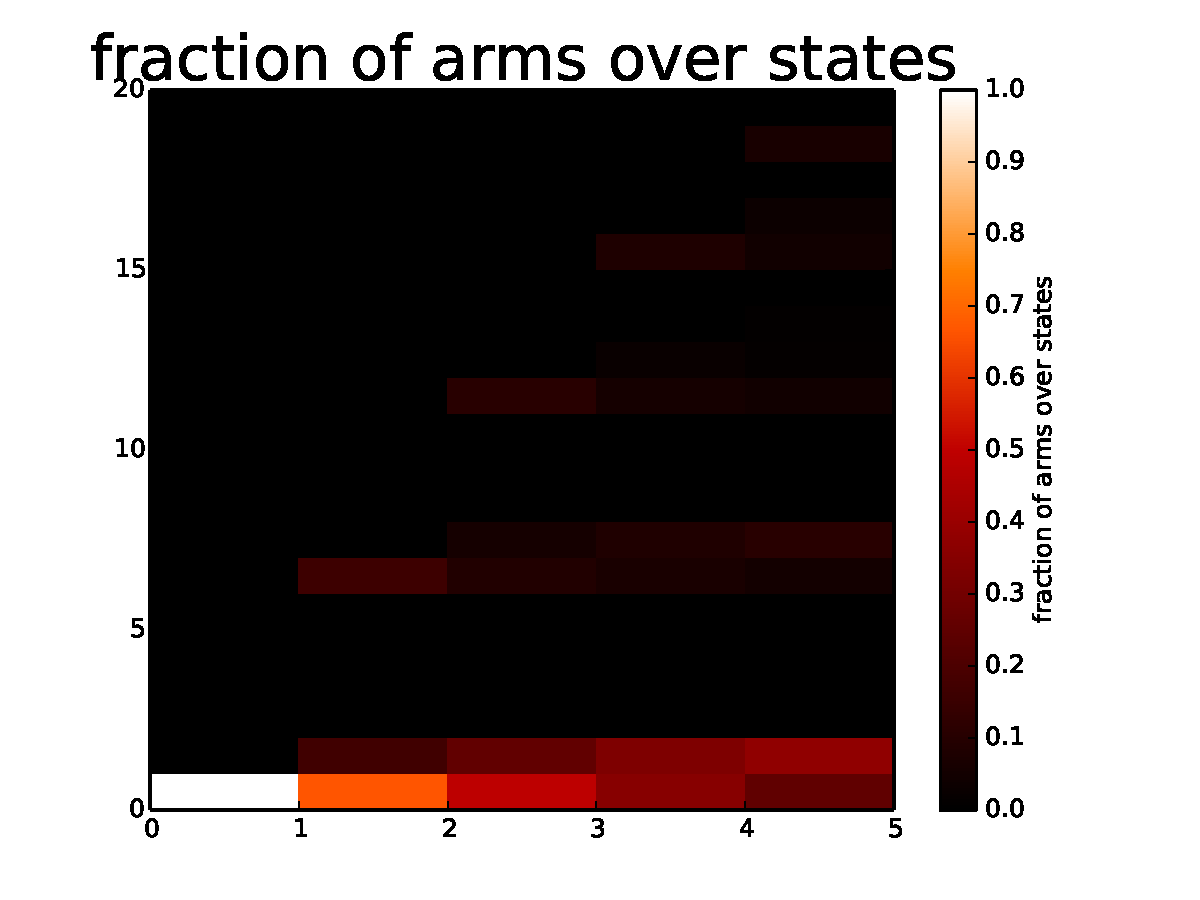
\includegraphics[width=45mm]{heat_map_index_s.pdf}}}
\only<1>{\subfigure{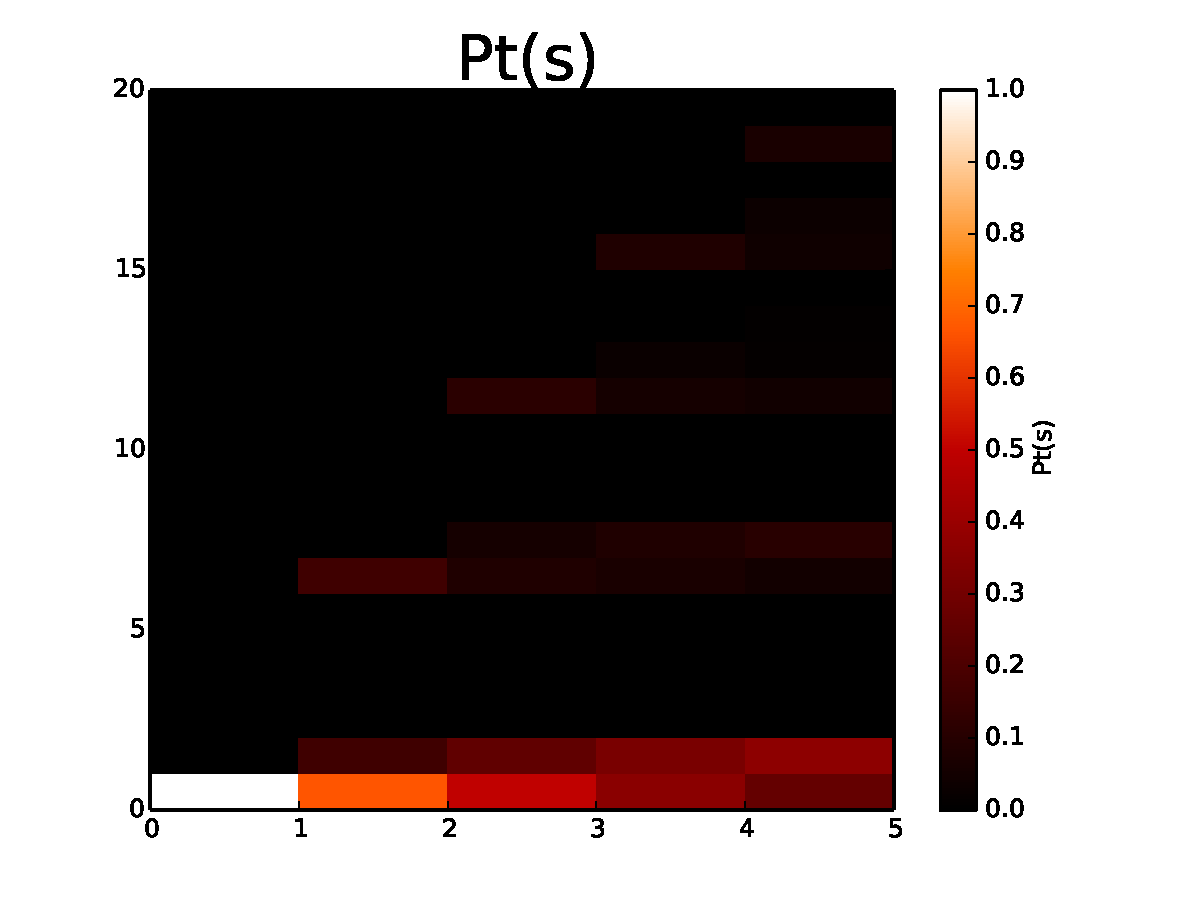
\includegraphics[width=45mm]{heat_map_pistar_s.pdf}}}
\only<1>{\subfigure{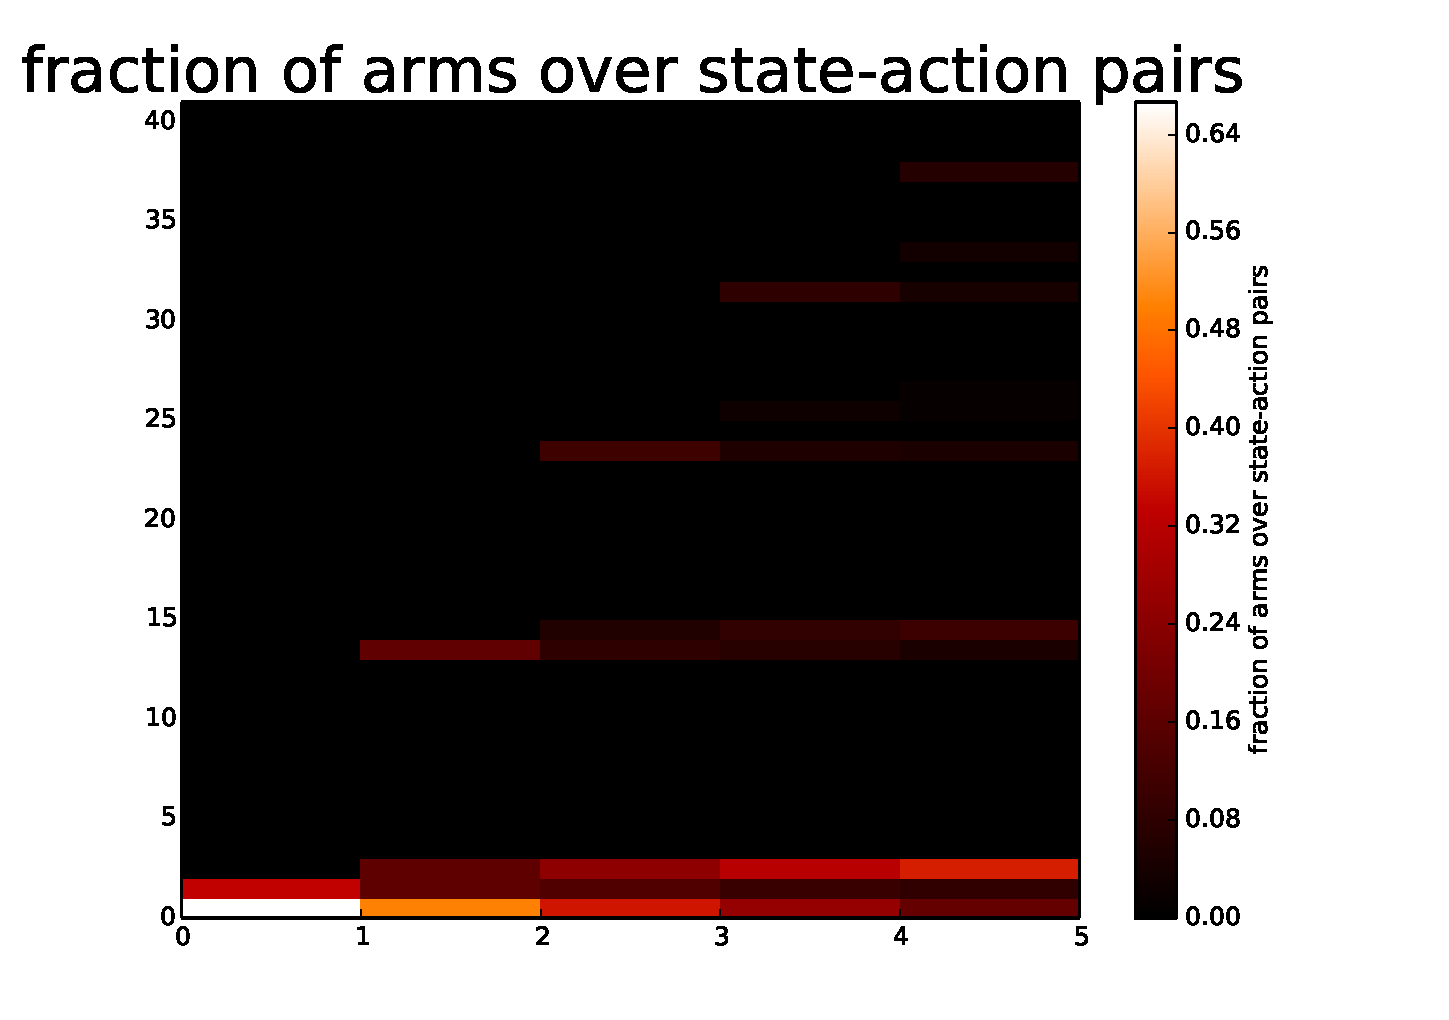
\includegraphics[width=45mm]{heat_map_index_sa.pdf}}}
\only<1>{\subfigure{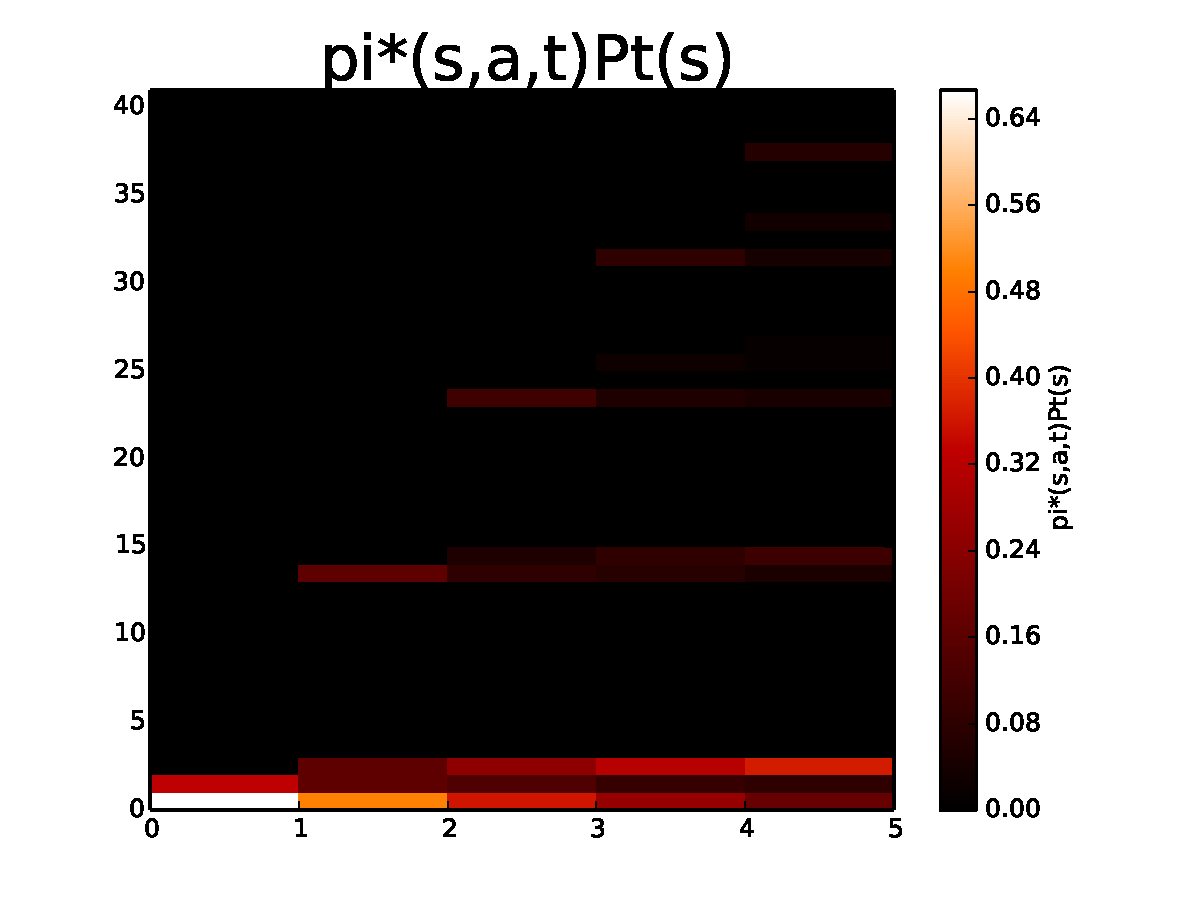
\includegraphics[width=45mm]{heat_map_pistar_sa.pdf}}}
\only<2>{\subfigure{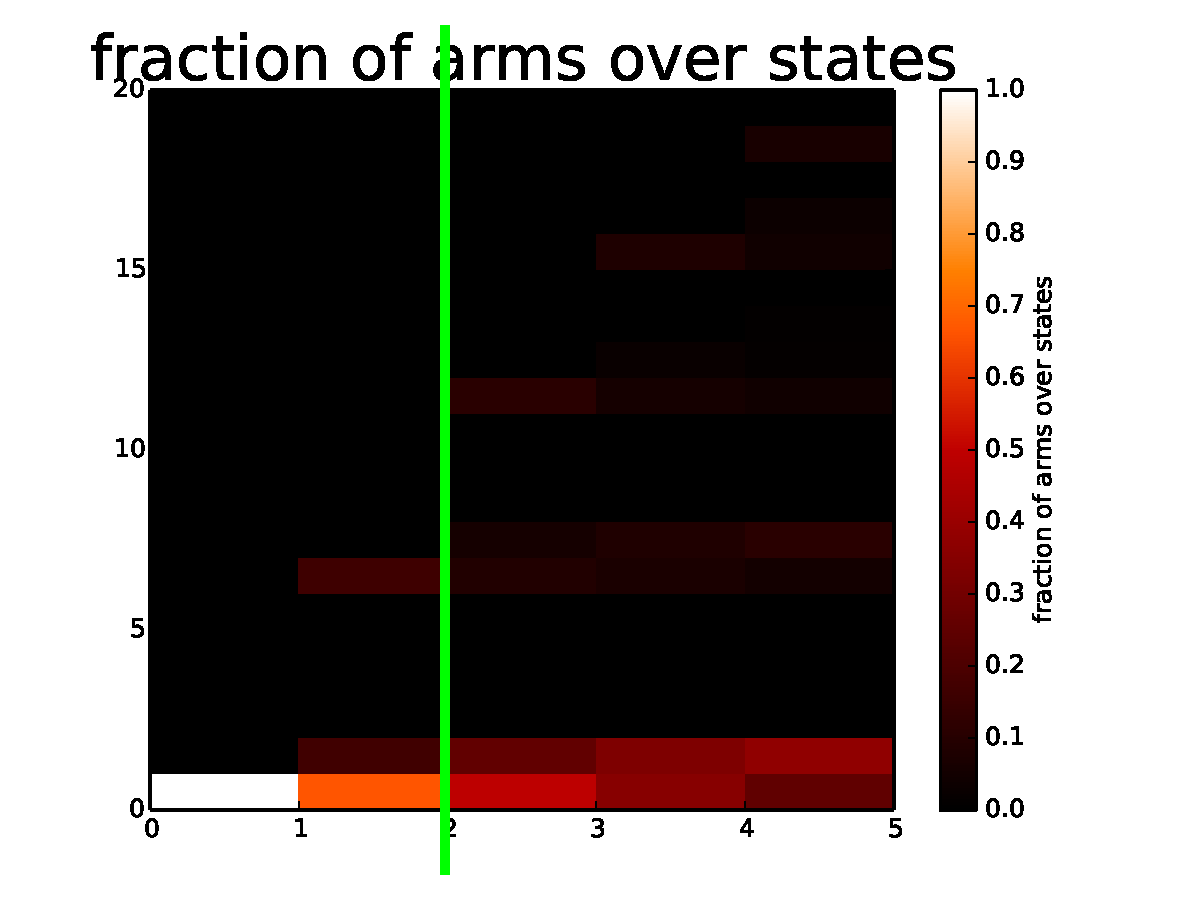
\includegraphics[width=45mm]{heat_map_index_s_lined.pdf}}}
\only<2>{\subfigure{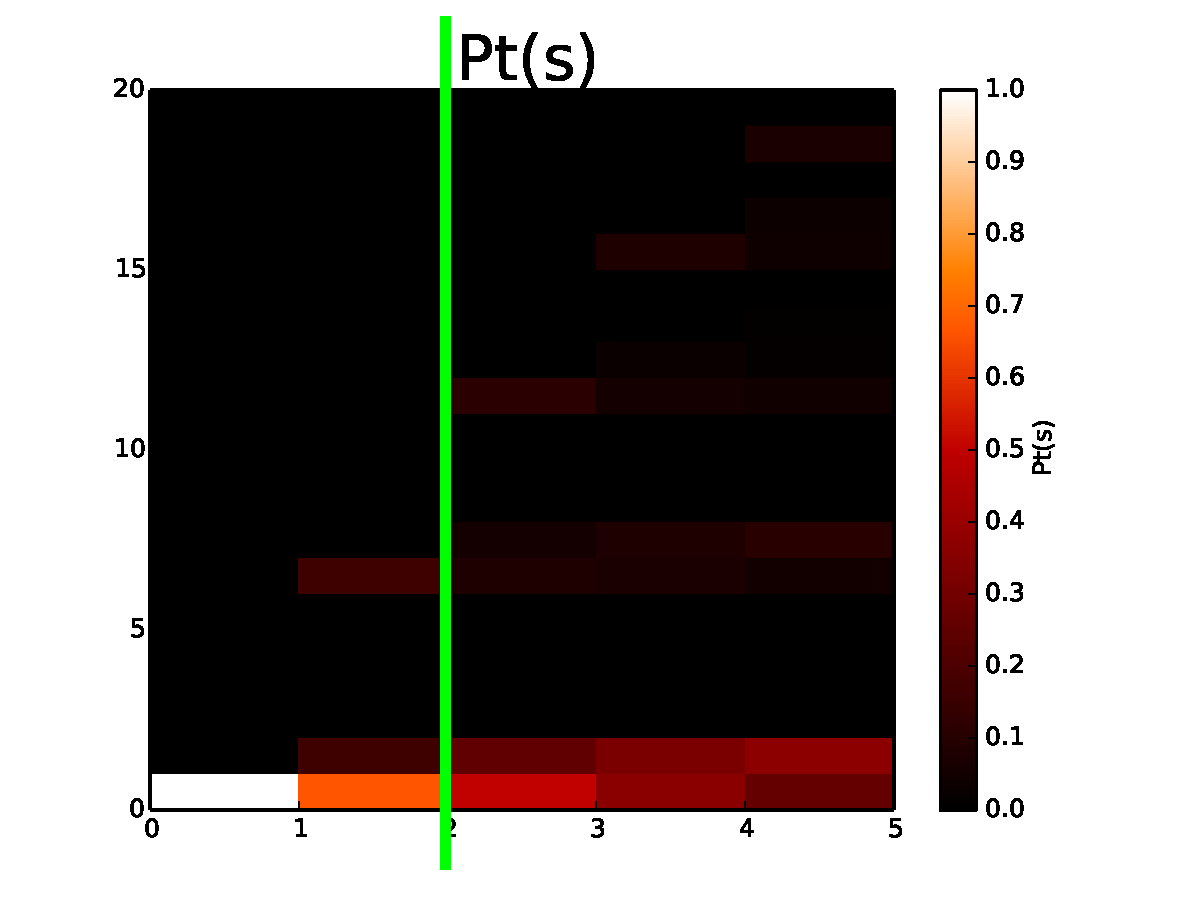
\includegraphics[width=45mm]{heat_map_pistar_s_lined.pdf}}}
\only<2>{\subfigure{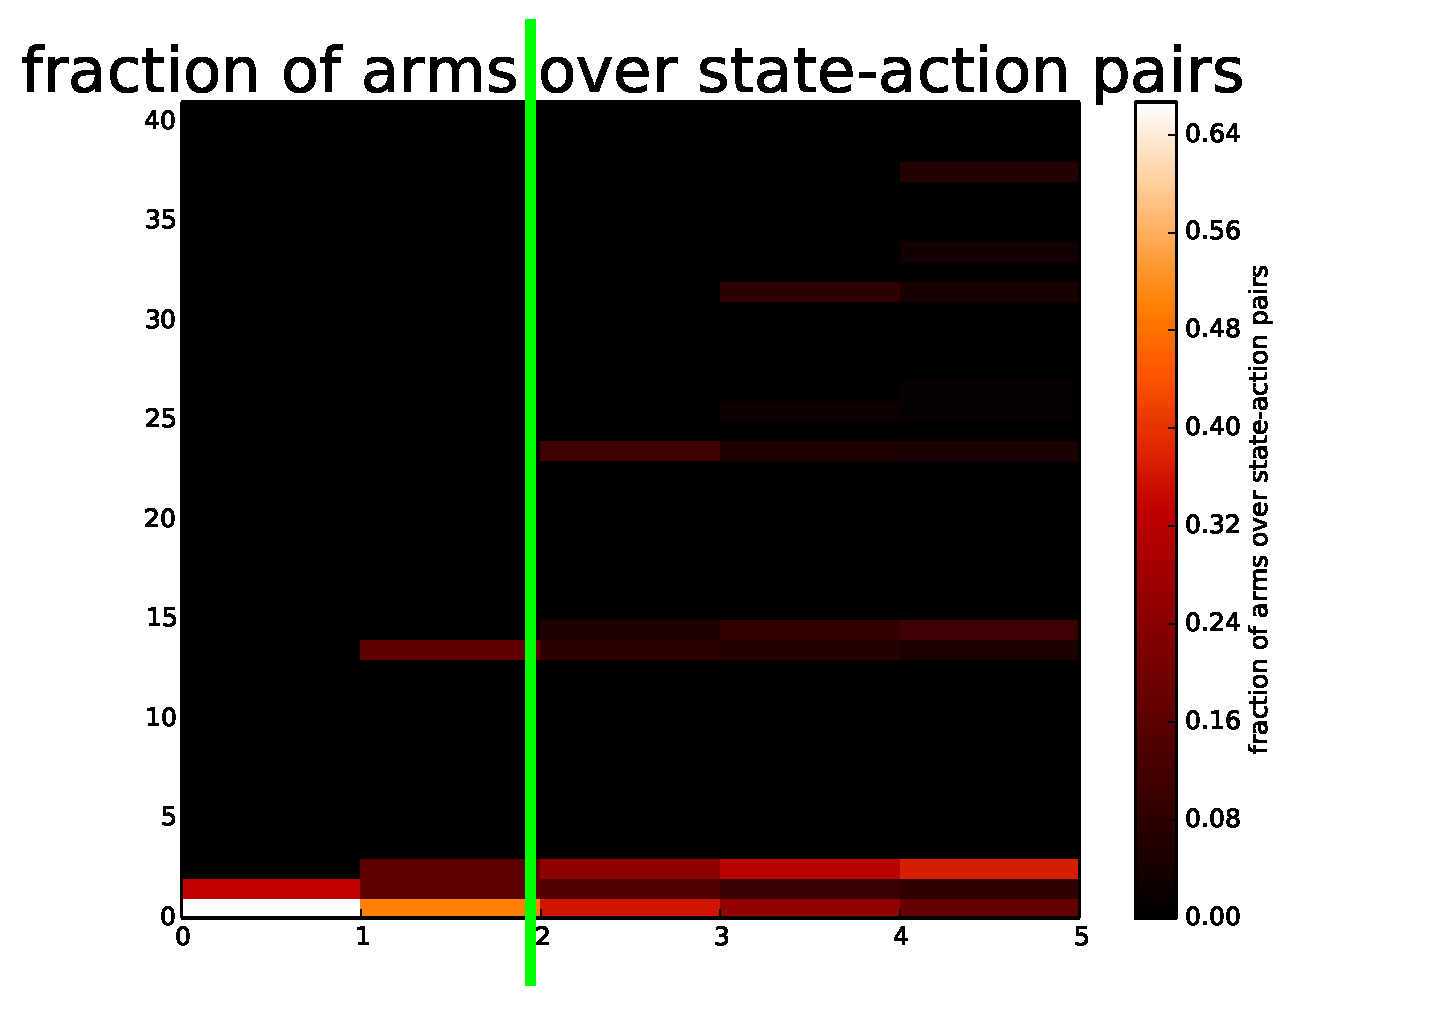
\includegraphics[width=45mm]{heat_map_index_sa_lined.pdf}}}
\only<2>{\subfigure{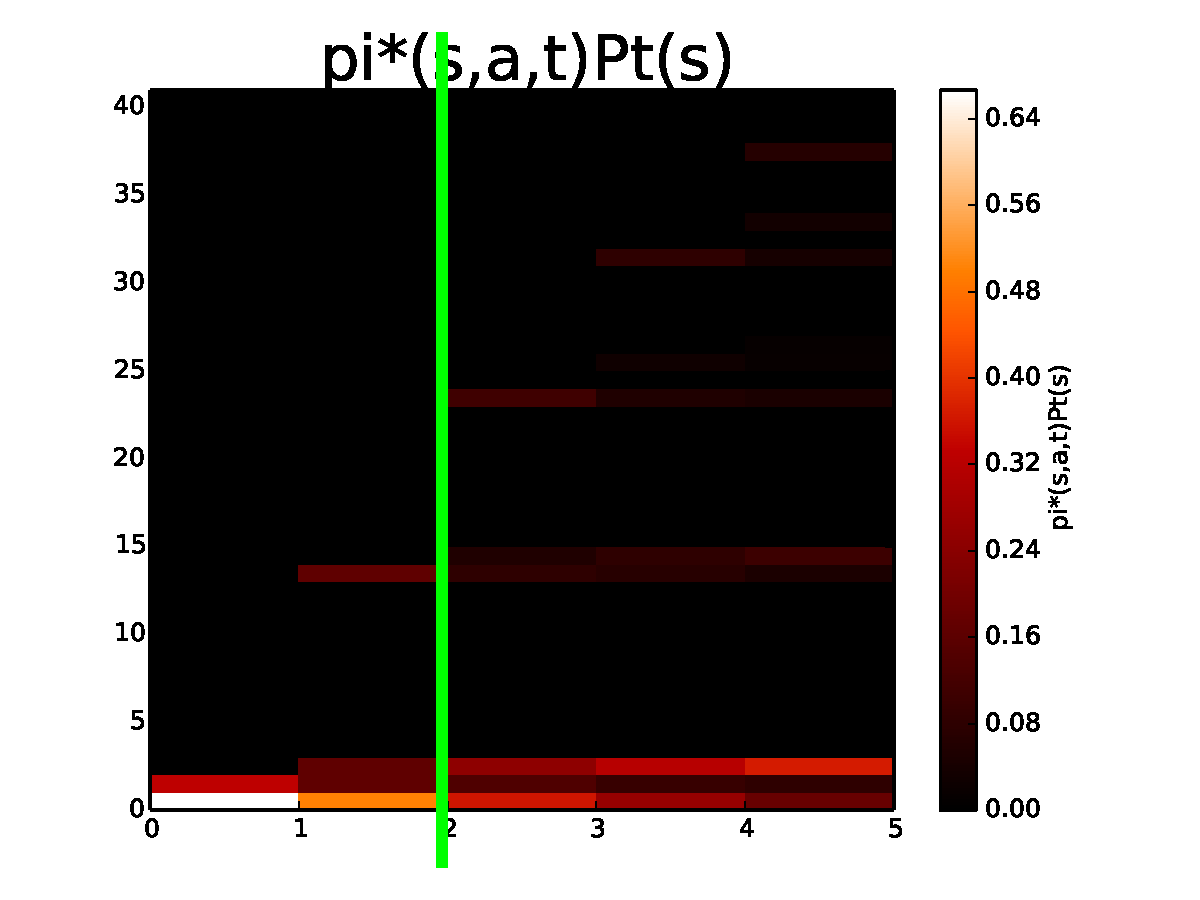
\includegraphics[width=45mm]{heat_map_pistar_sa_lined.pdf}}}
\end{figure}
\end{frame}
%%%%%%%%%%%%%%%%%%%%%%%%%%%%%%%%%%%%%%%%%%%%%%%%

%%%%%%%%%%%%%%%%%%%%%%%%%%%%%%%%%%%%%%%%%%%%%%%%
\begin{frame}
\frametitle{Proof of Theorem 1}
That $\hat{\allp}$ being feasible implies $$Z(\hat{\allp},\lfloor \alpha K\rfloor,K) \leq \max_{\allp\in\allpset_{\lfloor \alpha K\rfloor,K}}Z(\allp,\lfloor \alpha K\rfloor,K)$$.  Thus,
\begin{equation*}
\lim_{K\rightarrow\infty}\frac{1}{K}Z(\hat{\allp},\lfloor \alpha K\rfloor,K) \leq  \lim_{K\rightarrow\infty}\frac{1}{K}\sup_{\allp\in\allpset_{\lfloor \alpha K\rfloor,K}}Z(\allp,\lfloor \alpha K\rfloor,K).
\end{equation*}
\end{frame}
%%%%%%%%%%%%%%%%%%%%%%%%%%%%%%%%%%%%%%%%%%%%%%%%

%%%%%%%%%%%%%%%%%%%%%%%%%%%%%%%%%%%%%%%%%%%%%%%%
\begin{frame}
\frametitle{Proof of Theorem 1 Cont'}
On the other hand,
\footnotesize
\begin{align*}
\lim_{K\rightarrow\infty}\frac{1}{K}Z(\hat{\allp},\lfloor \alpha K\rfloor,K) 
=&\lim_{K\rightarrow\infty}\frac{1}{K}\Eb^{\hat{\allp}}\left[\sum_{t=1}^{T}\sum_{s\in\substates}r_t(s,1) M_{t}(s)+r_t(s,0) (N_{t}(s)-M_{t}(s))\right]\\
=&\sum_{t=1}^{T}\sum_{s\in \substates}\left[r_t(s,1) \rho(s,1,t)+r_t(s,0) \rho(s,0,t) \right]\\
&\;\;\;\;\;-\mathbb{E}^{\subp^*}\left[\sum_{t}\lambda^*_t \left(A_t-\alpha_t\right)\right]\\
=& Q(\lambdav^*)+\alpha \sum\lambda^*_t\\
=& \lim_{K\rightarrow\infty}\frac{1}{K}(KQ(\lambdav^*)+\lfloor \alpha K \rfloor\sum\lambda^*_t)\\
=& \lim_{K\rightarrow\infty}\frac{1}{K} P(\lambdav^*,\lfloor \alpha K \rfloor, K)\\
\geq& \lim_{K\rightarrow\infty}\frac{1}{K}\sup_{\allp\in\allpset_{\lfloor \alpha K\rfloor,K}}Z(\allp,\lfloor \alpha K\rfloor,K).
\end{align*}
\end{frame}
%%%%%%%%%%%%%%%%%%%%%%%%%%%%%%%%%%%%%%%%%%%%%%%%
\end{document}










